\chapter{Design}

\TODO{INTRO}


\section{System Architecture}

\TODO{High-Level description and block diagram}

\begin{figure}[!ht]
		\centering
		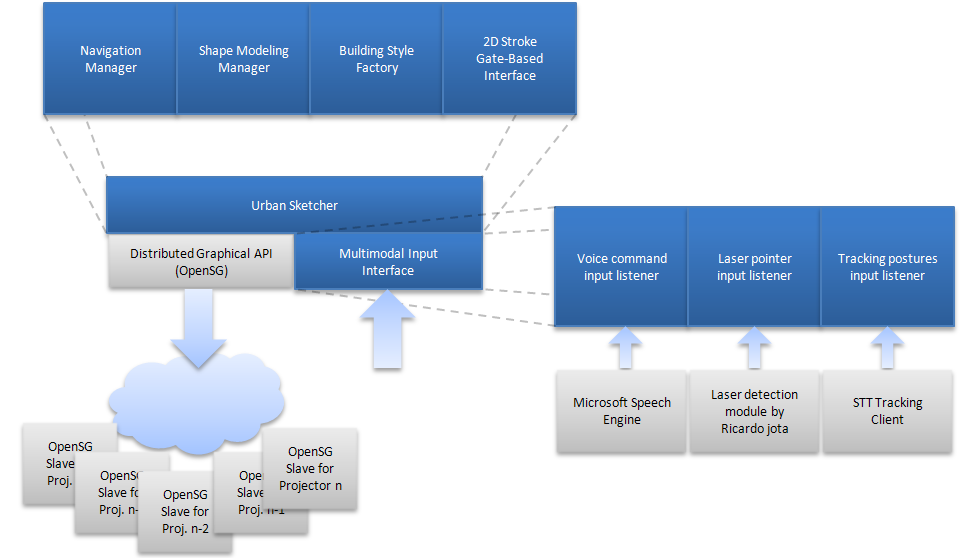
\includegraphics[width=17cm]{gfx/charts/block-diagram.png}
		\caption{Urban Sketcher Architecture Diagram}
		\label{fig:block-diagram}
\end{figure}

\TODO{REMOVE 'ricardo jota'; add mouse input; add broadcast and remove input arrow}

Urban Sketcher has at its core the following items\footnote{Blue items denote work done by the author.}:

The \textbf{Navigation Manager} is
		responsible for assembling navigation data from
		both voice and tracking input plus gate events which trigger navigation changes,
		supporting several navigation modes;
	
The \textbf{Shape Modeling Manager} is
		responsible for representing a 3D editable shape
		along with its geometry information, range of operations and a
		Memento Pattern for supporting undo operations;
	
The \textbf{Building Style Factory} is
		responsible for parsing building style definitions
		and converting blueprints and height to actual building instances;
	
The \textbf{2D Stroke-Based Interface} is 
		a set of interface widgets and their controllers,
		supporting option gates, ring menus and stroke-based operation handling.
Urban Sketcher gets input from several media:
laser pointers, the server machine's mouse and optionally voice commands and tracking postures.
The system can render real-time views to any number of slave machines.
An XML configuration allows parameterizing the range of affected machines and topology of the rendering slaves,
allowing the own machine to work as slave, a set of remote machines or both.


\section{Stroke-Based Input Interface}

This section details the concepts used in the creation of the interface for the system.

\subsection{Strokes}

A stroke is the result of continuous input from one laser pointer, from the time the laser
light button is pressed until it is released. 

By using the laser detection module, the system gets a stream of laser readings which
come sequentially tagged, that is, the module identifies with reasonable success when different strokes
occur simultaneously, returning both readings tagged with different stroke IDs.
Even so, the module can't infer whether different strokes came from the same source laser pointer.

This limitation sets an important assumption in our system -- one can not know whether 2 strokes came
from the same user, therefore operations must take place during at most the stroke period.

Strokes can also be emulated by using a mouse and pressing
the button as if it were a laser pointer.


\subsection{Gates}

The most common activation action in current Graphical User Interface (GUI) computer interactions works
by displaying a button on the screen and the user activating it by pressing the pointer device button.
Given that users will rely on laser pointers to interact with the GUI, a limitation derives from
using them instead of mice or track balls -- while a user isn't pressing the laser light button,
neither the system nor the user himself can know accurately where on the screen the laser is pointing to.
In order for the user to see the laser projection on the screen he must be pressing the button.
This necessity \TODO{urges} for a different GUI solution.

Based on prior research by \cite{CROSSY}, the gate concept was implemented with slight changes.

A gate is an imaginary two dimensional line on the screen, bound by two visible extremes.
To activate it one must draw a stroke which crosses the line, as if scoring a goal.

Gates can have a text label or a suggestive image to symbolize the action they perform.
It was decided not to mix both representations -- if the gate is illustrated, a tooltip can be invoked
by approaching the gate's area of influence without crossing it, so the action can be avoided.

\TODO{IMAGE ACTIVATION GATE}


\subsection{Menus}

\TODO{REVIEW TEXT...}
The menus in this system are ring-shaped, with the options (gates) organized along the ring.
Menus aren't totally opaque so the main viewport remains visible and each menu's background color
depends on the functionality it offers. On the bottom-right area a label identifies the functionality.
The top-right area features some additional gates so the menu can be dismissed, moved around and
returning to the main menu in possible.

A lot of effort has been put for menus to be usable. On cases where menus offered a large number of actions/options,
those were clustered into modes to keep a conveniently small number of visible options.
On such menus, selecting different modes is a matter of activating one of the left-side illustrative gates.

Submenus are another way of clustering options. \TODO{...}

\TODO{MENU WITH CAPTIONS, MODES, DRAG?}



\subsection{Strokes Gestures}

To invoke the main menu the user needs to draw a closed triangle stroke.
When that occurs the menu appears centered on the stroke just drawn.

\TODO{MAIN MENU STOKE, TREE OF MENUS}

Besides menus deriving from the main menu tree, which is invoked as we've just seen by drawing a closed triangle stroke,
there are menus which focus on an existing shape on the 3D world.
These are called contextual menus and they can be invoked by selecting the desired shape's face or edge.

To select a face one has to draw a small stroke starting and ending inside the face.

To select an edge one has to draw a small stroke starting on one of the edge's neighboring faces and ending at the remaining one,
effectively crossing the edge to select it.

\TODO{FACE AND EDGE SELECTION}


\section{Multimodal Input Interface}

Using laser input allows to explore all the system functionality.
Even so, an alternative arm-tracking and speech recognition command interface exists to enhance particular tasks.
The arms are tracked by attaching 2 reflective markers on each arm: one on each wrist and one close to each elbow.
Speech commands are obtained from a wireless headset attached to the user's ear.

\TODO{REFLECTIVE MARKETS / HEADSET FIGURE}

\subsection{Arm Posing Flight Mode}

This is an alternative navigation mode. Since it affects the point of view, this task can't be performed by
several people simultaneously, therefore unlike most of the system this navigation mode has global states
-- the user might be either stationary of flying.

The user starts interacting by having his arms extended toward the screen.
In order to begin flying the command ``Begin flying'' must be given.
To stop at any time one only needs to say ``Stop flying''
\footnote{Although semantically inconsistent, the words begin and stop were used after performing speech recognition
tests with both start/stop, begin/end and begin/stop, concluding that this combination had the better recognition ratio}.

Controlling flight speed works by measuring the distance between hands -- the closer they are to each other, the faster
the flight speed is. If the arms does a wide enough angle the flight comes to an halt.
Changing the flight orientation relatively to the ground is achieved by setting the arms angle with the ground at opposing directions,
with a bigger difference between these angles generating a faster rotation movement. If the user wants to turn right, for instance,
he has to raise the let arm and lower the right one.

To change the flight altitude, both arms must be oriented in the same direction relatively to the ground plane
-- either both raised or lowered. Again, the higher the angle is from the original forward pose position,
the bigger the flight altitude shirt is.

\TODO{INSERT FLIGHT FIGURES}


\section{Content Creation Concepts}

\subsection{Apply-to-Scene Creation}

To create a new object on the scene one has to perform a stroke which activates the desired shape design gate (cube for instance)
and continue the stroke onto the desired location where the shape should rest. As soon as the gate is activated, the shape appears
on top of the stroke and keeps following the stroke until it ends, offering a preview of the location where is would rest
if the stroke ended that particular moment.
To figure out the actual location for the shape during the task, the shape is collided in real-time against the
existing scene geometry so it stays in touch with the environment.

\TODO{FIGURE APPLY-TO-SCENE}


\subsection{Instancing a Building}

To create a building one has to feed the system 3 parameters: building style, blueprint and height.
Due to the system decision for stroke-driven actions without global state, these 3 parameters are given with the
minimum strokes (2), as described next.
From a menu the list of supported building styles is presented to the user, each style a different gate.
Once activating the desired style the user starts an apply-to-scene process, moving a construction plane which must
be put where the blueprint is to be drawn.
The user draws a closed rectangle representing the blueprint and after closing it continues
the stroke upwards in order to define the building height.
Once the stroke ends the building is generated according to the given parameters.
The construction plane has carried out its purpose and therefore is terminated.


\TODO{FIGURES BUILDING CREATION}